\section{Human Data}
\subsection{Data Quality}

Visualization in mode-maps gives qualitative confirmation that the data and the cleaning procedure give reasonable information about the color lexicon of the respective languages (Fig. \ref{fig:color_maps_english}).
Overall, we found the split-half ARI value for all languages to be high (range=.66-.88, mean=.75 sd=.05, Tabl.: \ref{tab:pgfplotstable_csv}).


\subsection{Comparison between Recruiters}

 Figure \ref{fig:color_maps_english} shows the English proportional maps obtained from Prolific and Lucid and compares them to the maps by \textcite{lindseyColor2014} (data reproduced with permission). 
We found a high ARI between \textcite{lindseyColor2014} and Prolific and Lucid (.72 [.67, .77] and .67 [.62, .72], respectively, CIs via bootstrapping, Fig. \ref{fig:color_maps_english}). 
For other languages that were tested on both recruiters (English, Italian, and Greek), the ARIs were also high (.70 [.65, .74], .61 [.56, .66], and .63 [.57, .68], respectively, (Fig. \ref{fig:color_maps_english}). 

 % In these maps, each chip is colored by the majority vote for this particular chip. We plot the color of the region associated with a term to be the average color (in RGB space) across all winning chips. 
 As indicated by the legends, participants mention similar color categories which cover similar proportion of chips across the data sets.
 The prolific sample includes two newly emerging color terms 'lilac' and 'teal' which are already discussed by \textcite{lindseyColor2014}.
 Majority vote over all participants on Lucid converged on the 11 basic color categories proposed by \textcite{berlinBasic1969} with white as one exception.
 Interestingly, throughout our dataset we see a consistently small or utterly absent white category. This is most likely due to the way we present the stimulus (Fig. \ref{fig:col-trail}). The square of color is presented on a white page. When showing very light chips a side effect might be that they never meet exactly the white of the page right next to the stimulus. The task undeliberately turns into a distinction task which makes it easy for people to see the very light color instead of just white.

 

\begin{figure*}[h!t]
    \begin{center}    
    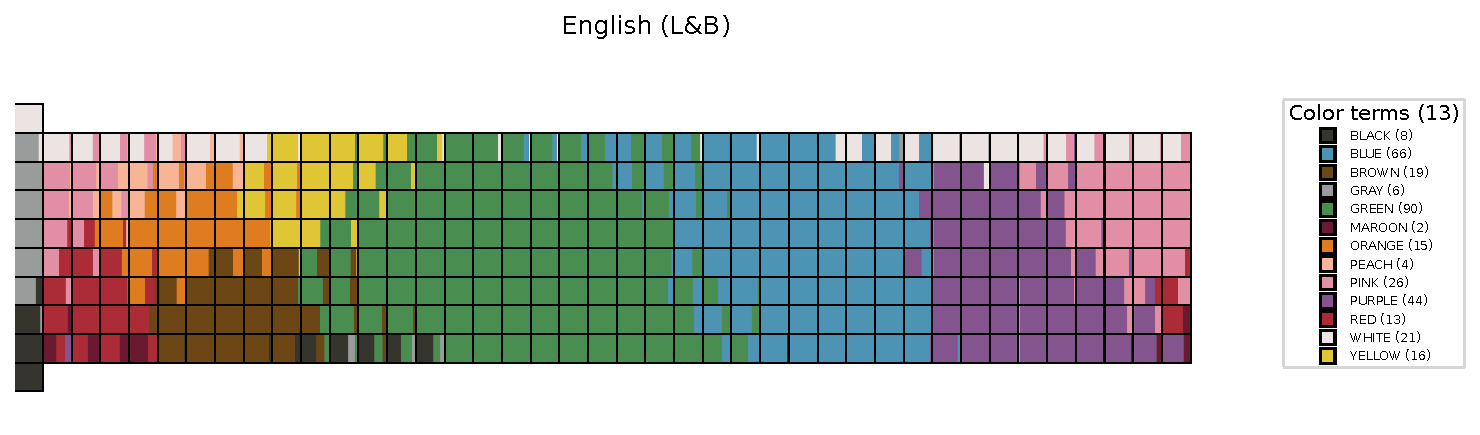
\includegraphics[page=1, width=\linewidth]{images/mode_maps/English (L&B).pdf}
    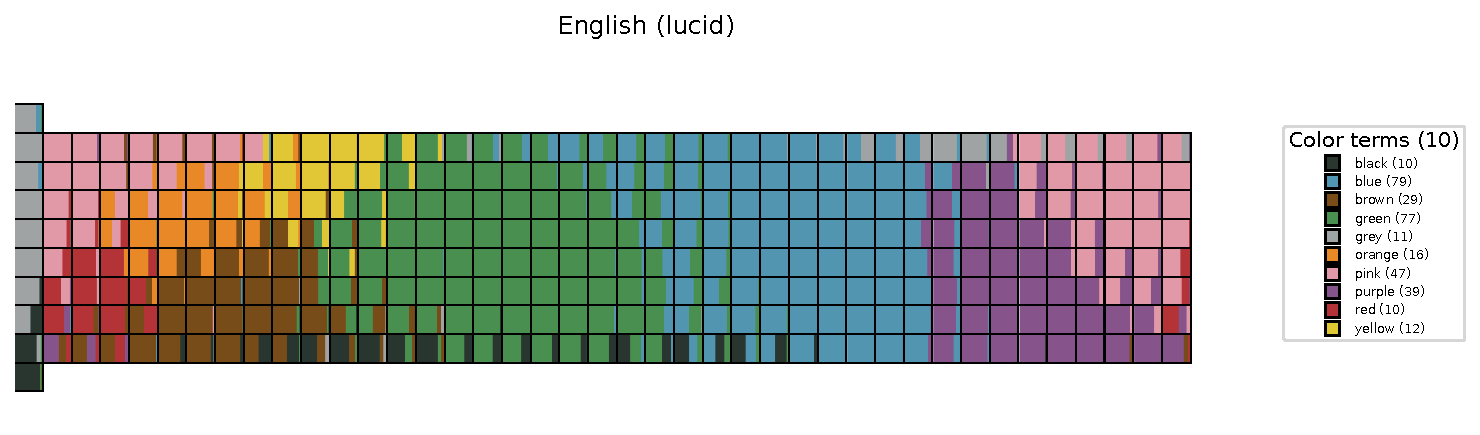
\includegraphics[page=1, width=\linewidth]{images/mode_maps/English (lucid).pdf}
    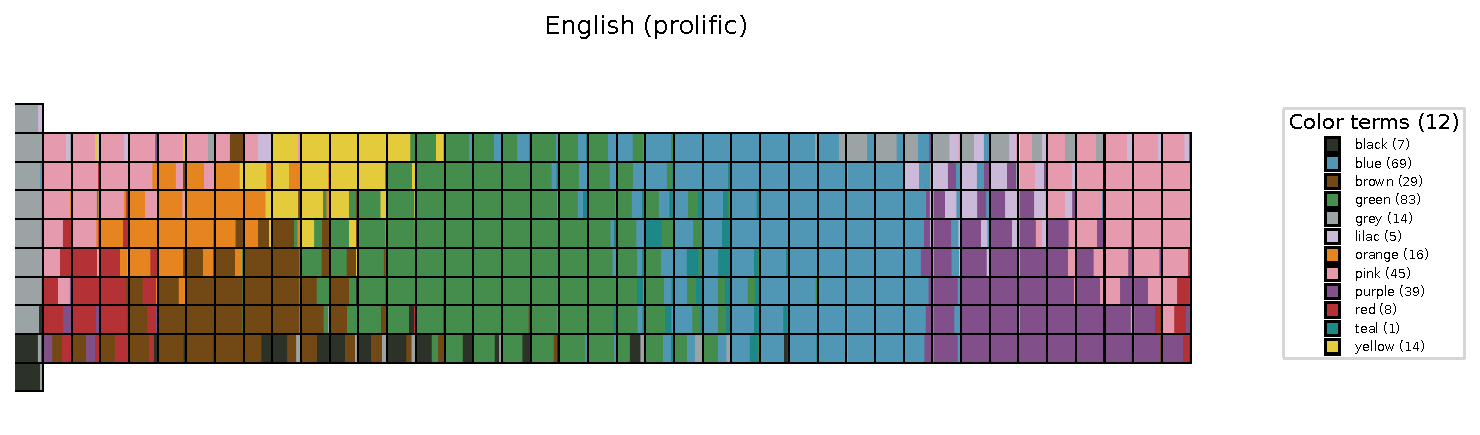
\includegraphics[page=1, width=\linewidth]{images/mode_maps/English (prolific).pdf}
    \end{center}
    \caption[English Proportional maps]{English Proportional maps: Upper panel: Reproduction of data from an in lab experiment by \textcite{lindseyColor2014} with permission. Middle and lower panel: Newly online collected Data on different recruiters Prolific and Lucid.
    Proportional maps show qualitatively high accordance across the different occasions of data collection.}
    \label{fig:color_maps_english}
\end{figure*}

\begin{figure*}[h!t]
    \begin{center}    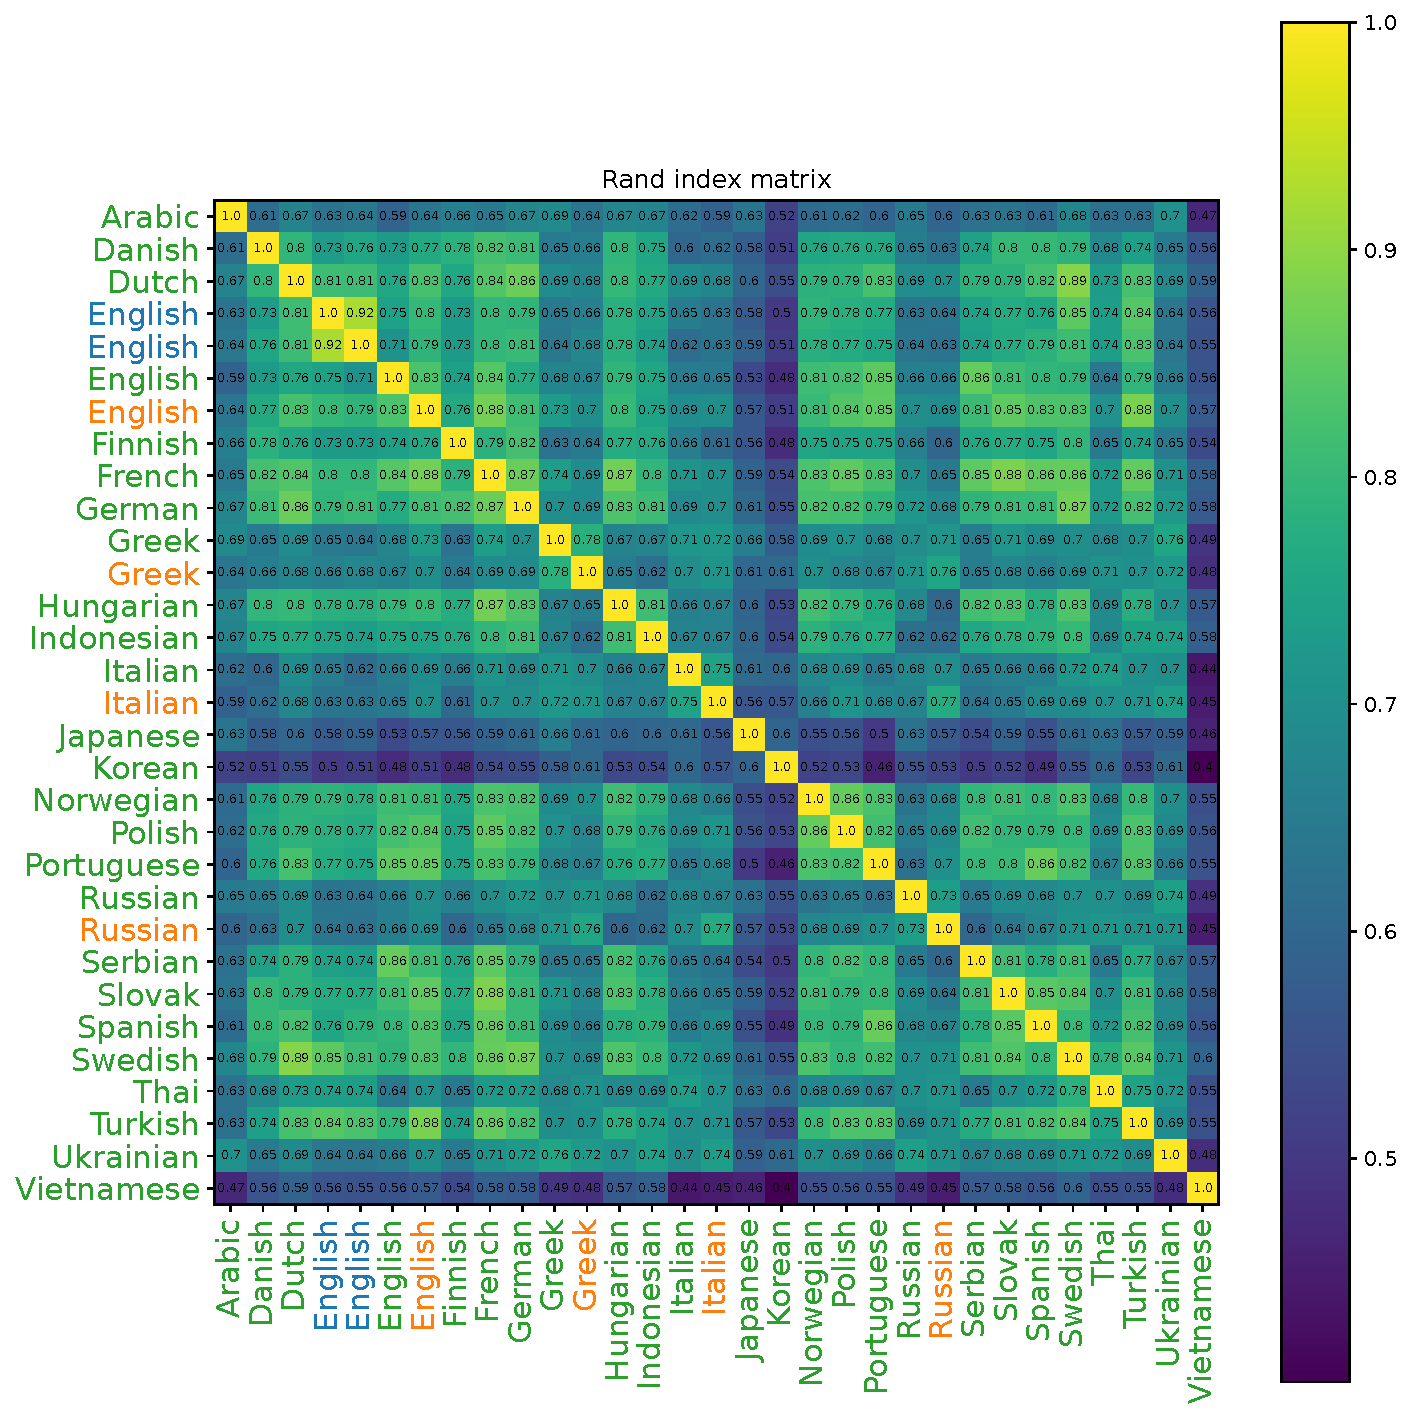
\includegraphics[width=\textwidth,height=\textheight,keepaspectratio]{images/rand_index_matrix_all.pdf}
    \end{center}
    \decoRule
    \caption[Rand Index Matrix human data]{Rand Index Matrix for human data from \textcite{lindseyColor2014} (blue) and newly collected data on recruiters Prolific (orange) and Lucid (green). Rand index indicates similarity of naming pattern of respective languages, ranging from 1, exactly the same, to 0, dissimilar clustering.}
    \label{fig:rand_index_matrix}
\end{figure*}


\subsection{Comparing to WCS Data}

% Mean ARI (Uniformness of the dataset)
Compared to the WCS languages the collected dataset seem more homogeneous.
The mean ARI across the entire dataset is .70 [.50, .89] whereas it is much lower across the WCS languages (.43 [.18, .68]).
Across both data sets, the mean ARI is significantly lower .31 [.05, .57] than within the two data sets (p<.001 for both cases via the Mann-Whitney U test), confirming the difference.
% Number of Color Term
Significant distinction was also found for the number of color terms which was higher in the Lucid dataset (9.02 [5.92, 12.12]) than for the WCS data (5.71 [2.57, 8.85], p<.001 via the Mann-Whitney U test).
The number of color terms here is calculated by computing the exponent of the entropy on all chips.
The variance of the number of color terms was equally high in both data sets.


\subsection{Analysis of Single languages}

\paragraph{English:}
\textcite{berlinBasic1969} claimed to have found eleven basic color categories represented by the 11 English color categories \textit{black, white, red, yellow, green, blue, brown, orange, pink, purple, and gray}.
The English data elicited on Lucid reproduced this list of color terms with one exception: white.
Because of the high concordance with the literature the English data will be used as a reference when analysing other languages.
(Split-half-rand-index = 0.85)

\paragraph{Arabic:}

We found a relatively broad lexicon for Arabic, namely 18 winning color terms. Interestingly, there is a distinction in the blue category differentiating \textit{light blue} from \textit{dark blue}.
Furthermore, many color terms are derived from objects such as the word for \textit{grey}
\begin{Arabic}رمادي\end{Arabic}(ramadi), coming from \begin{Arabic}رماديرماد\end{Arabic}(ramad), which means ashes or \begin{Arabic}رصاصي\end{Arabic}(rṣaṣi) translates to lead.
The data show a relatively large white category of six chips. (Split-half-rand-index = 0.66)


\paragraph{Danish:}
% hvid} (2)
Aligns to the English color lexicon covering all BCT.
Interestingly, we see a \textit{white} category of only small size covering two color chips.
(Split-half-rand-index = 0.74)

\paragraph{Dutch:}
The dutch color lexicon contains apart from \textit{white} all eleven BCT plus one additional small \textit{lila} category and a double category for \textit{roze} which was not caught by our cleaning algorithm.
Here the \textit{white} category is entirely absent. 
(Split-half-rand-index = 0.76)

\paragraph{Finish:}
Finish data show all BCT plus a \textit{lila} and \textit{turkoosi} category.
Here the \textit{white} category wins in 3 chips.
(Split-half-rand-index = 0.73)

\paragraph{French:}
French data show high accordance with the BCT. However the white category only covers 1 chip.
(Split-half-rand-index = 0.81)

\paragraph{German:}
In addition to the BCT which are all present in the German data ocker \textit{türkis} and \textit{beige} are introduced as additional color terms.
(Split-half-rand-index = 0.79)

\paragraph{Greek:}
Greeks belong to the languages differentiating between \textit{light blue} \textgreek{θαλασι} (thalassi) sea and \textit{dark blue} \textgreek{μπλε} (ble).
%\textgreek{λάχανο} (lachano) literally translates to cabbage and might have been used metaphorically for a color, but it's not a standard color term in Greek.
\textgreek{κιτρινοπο} seems to be a spelling which was conserved despite our cleaning procedure and represents the standard word for \textit{yellow} \textgreek{κίτρινο} (kitrino).
\textgreek{τιρκοθαζ} is the direct translation of \textit{turquise} into Greek letters but is not considered to be a native Greek word.
(Split-half-rand-index = 0.77)

\paragraph{Hungarian:}
The elicited color lexicon for Hungarian covers all BCT.
In addition we found a quite large category \textit{bordo} for \textit{dark-red}.
(Split-half-rand-index = 0.75)

\paragraph{Indonesian:}
The Indonesian color lexicon includes all BCT plus one small category krem.
A small \textit{white} category is present as well.
(Split-half-rand-index = 0.76)

\paragraph{Italian:}
Italian belongs to the list of languages making distinctions between \textit{blu} - \textit{blue} and \textit{azzurro }- \textit{light blue}. Interestingly, Italian possesses one additional category for blue: \textit{celeste} which means\textit{ very} \textit{light blue}.
\textit{Verdino} also shows up in the list which means \textit{greenish} but did not get caught by the cleaning procedure.
(Split-half-rand-index = 0.74)

\paragraph{Japanese:}
Japanese makes three distinctions in the blue category.
First, \japaneseText{アオ色} (ao-iro): basic \textit{blue} color. Second, \japaneseText{コン色} (kon-iro): \textit{navy blue} or \textit{deep blue} color. Third, \japaneseText{ミズ色} (mizu-iro): Water color, often referring to a clear, \textit{light blue}.
\japaneseText{ダイダイ色} (daidai-iro) represents a specific type of \textit{orange} color. Daidai refers to a specific shade of \textit{orange}, named after the bitter orange fruit.
\japaneseText{モモ色} (momo-iro) means \textit{peach}, \japaneseText{ハダ色} (hada-iro) \textit{skin color} and \japaneseText{ヒ色} (hi-iro) which is likely a typo or shorthand. If it meant to be \japaneseText{ヒワ色} (hiwa-iro), it would refer to a \textit{light yellow}.
All other color terms refer to the BCT named by Berlin and Kay with only white missing.
The relatively large color lexicon that we found is consistent with earlier studies that claimed to have found 16 statistically distinct color terms for Japanese \parencite{kurikiModern2017}.
(Split-half-rand-index = 0.73)

\paragraph{Korean:}
Korean possesses a very large color term lexicon. Interesting distinctions here are between \textkorean{파란색} (paransaek) - \textit{Blue} and 
\textkorean{하늘색} (haneulsaek) - \textit{Sky Blue}. 
Green is subdivided by three terms: 
\textkorean{녹색} (noksaek) Green
\textkorean{연두색} (yeondusaek) light green or lime green and
\textkorean{초록색} (choroksaek) another term for green, often used to describe nature.
The white category is missing.
(Split-half-rand-index = 0.47)


\paragraph{Norwegian:}
Norwegian color lexicon covers all BCT plus turkis and a double category for orange.
(Split-half-rand-index = 0.69)

\paragraph{Polish:}
All BCT present in the polish lexicon and two additional categories granatowy and bordowy. No white category here.
(Split-half-rand-index = 0.72)

\paragraph{Portuguese:}
Portuguese makes a profound distinction between lilás and roxo but does not report a white category.
(Split-half-rand-index = 0.81)

\paragraph{Russian:}
Most interestingly, Russian distinguishes between \textrussian{голубой} (goluboy) light blue or sky blue and \textrussian{синий} (siniy) which means blue.
Additional categories are: \textrussian{бордовый} (bordovyy): Burgundy and the distinction between \textrussian{сиреневый} (sirenevy): Lilac and \textrussian{фиолетовый} (fioletovyy): Purple
(Split-half-rand-index = 0.75)

\paragraph{Serbian:}
The serbian color lexicon coveres all BCT.
(Split-half-rand-index = 0.77)


\paragraph{Slovakian:}
Apart from the BCT slovakians inlude a small category for bordovy.
(Split-half-rand-index = 0.78)

\paragraph{Spanish:}
The data align very well to the english BCT but make a distinction between morado, lila and violeta in the purple region.
(Split-half-rand-index = 0.77)

\paragraph{Swedish:}
All BCT are covered by the Swedish lexicon plus one small category beige
(Split-half-rand-index = 0.74)

\paragraph{Thai:}
Contains all BCT apart from white, and makes distiction between \textthai{น้ำเงิน} (Nam ngern) blue and \textthai{ฟ้า} (Fa) sky blue or light blue.
(Split-half-rand-index = 0.76)

\paragraph{Turkish:}
Turkish basic color vocabulary covers all BCT with a very small white category and an additional small lila category.
Furthermore, it makes a distinction in the red area to dark-red bordo and dark blue lacivert.
(Split-half-rand-index = 0.74)

\paragraph{Ukrainian:}
We found a very comprehensive color vocabulary for Ukrainian with many small and specific categories.
Interesting however, is the large category for light-blue \textukrainian{блакитний} (blakytnyi) and light or lettuce and fresh green \textukrainian{салатовий} (salatovyi).
(Split-half-rand-index = 0.71)

\paragraph{Vietnamese:}
This is the only language we examined that does not cover all BCT. Vietnamese puts the green and blue category together in a grue category \textit{xanh}.
(Split-half-rand-index = 0.88)

% \paragraph{Summary:}
% Presence of a light blue category: Arabic, Greek, Italian, Japanese, Korean, Russian, Thai and Ukrainian.

% Presence of a blue category: Danish, Dutch, English, Finnish, French, German, Hungarian, Indonesian, Norwegian, Polish, Portuguese, Serbian, Slovakian, Spanish, Swedish, Turkish



\begin{figure}[htbp]
\centering
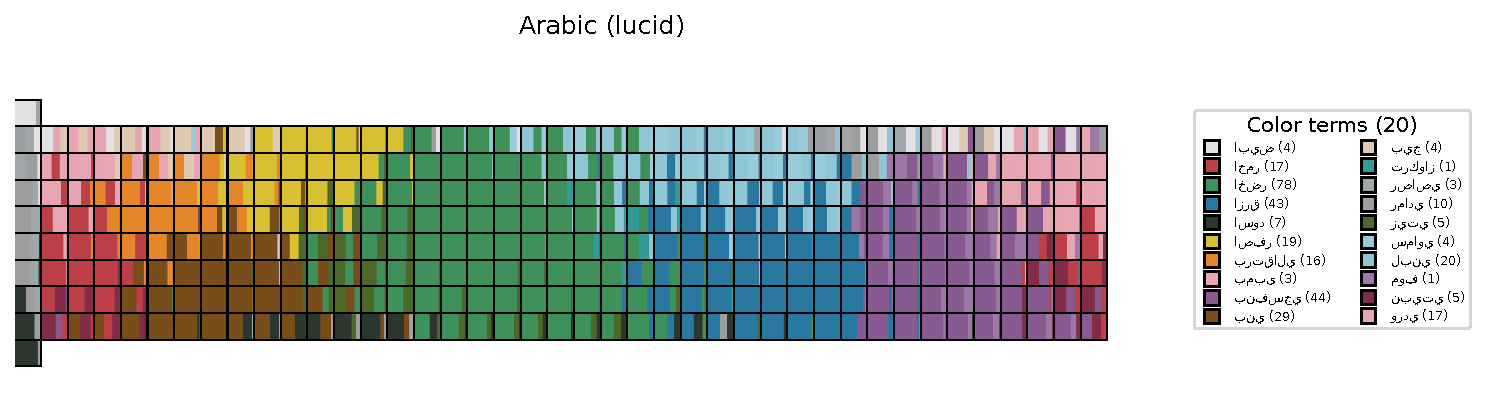
\includegraphics[page=1, width=\linewidth]{images/mode_maps/Arabic (lucid).pdf}
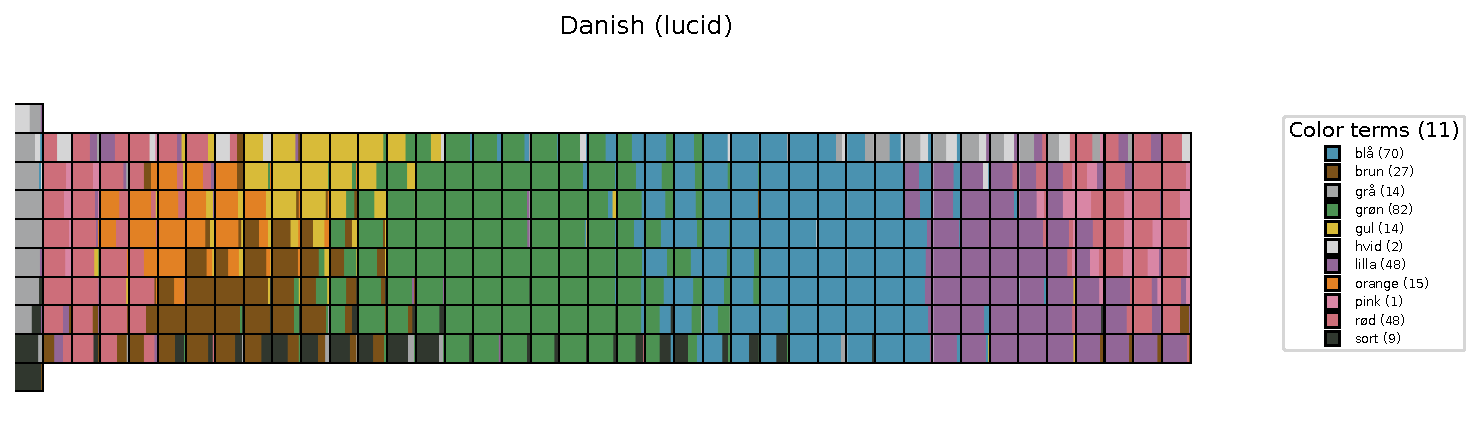
\includegraphics[page=1, width=\linewidth]{images/mode_maps/Danish (lucid).pdf}
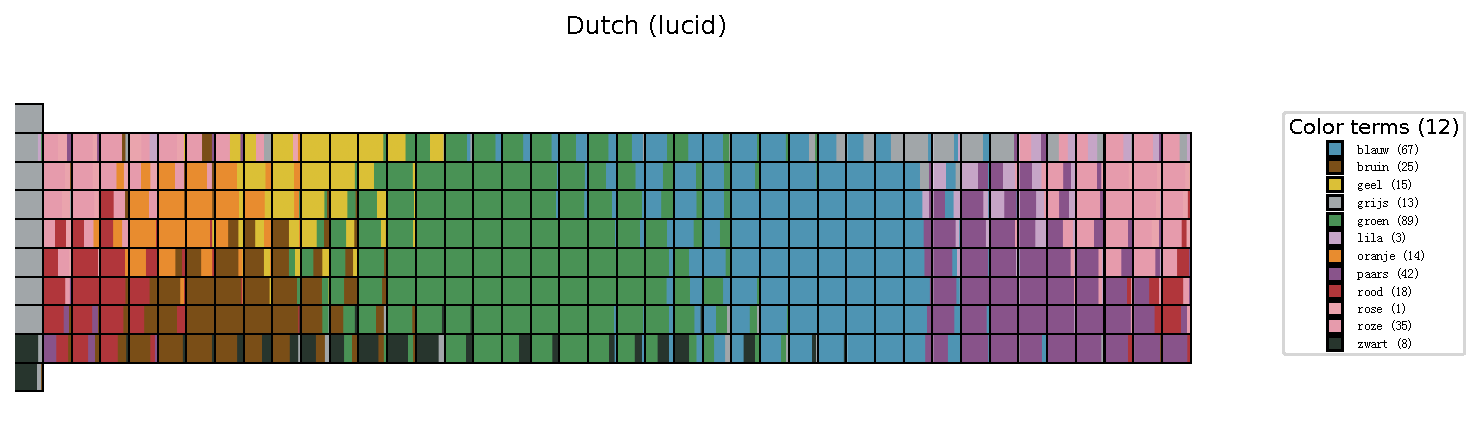
\includegraphics[page=1, width=\linewidth]{images/mode_maps/Dutch (lucid).pdf}
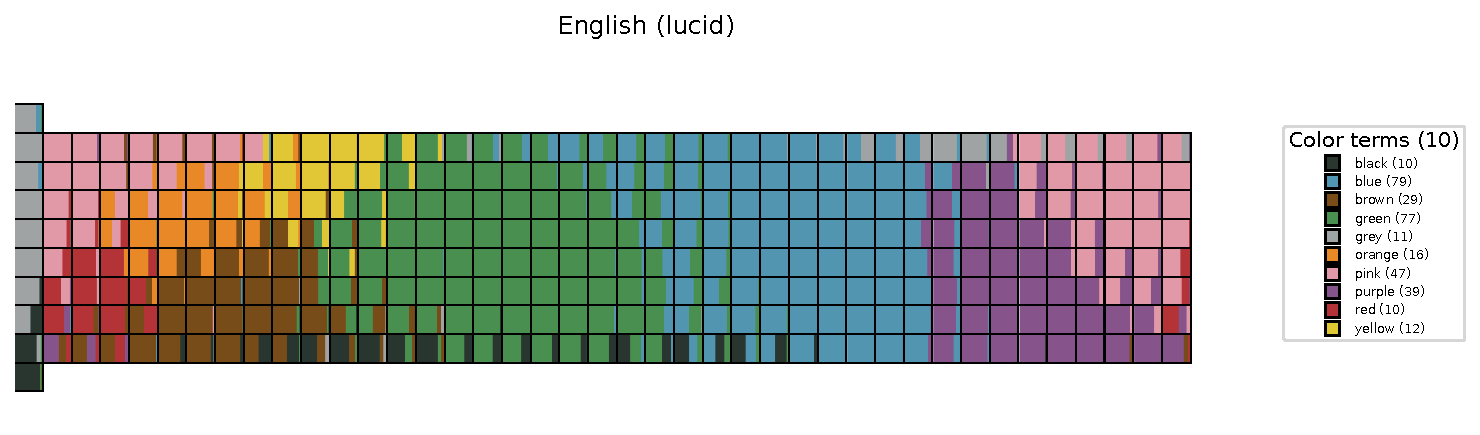
\includegraphics[page=1, width=\linewidth]{images/mode_maps/English (lucid).pdf}
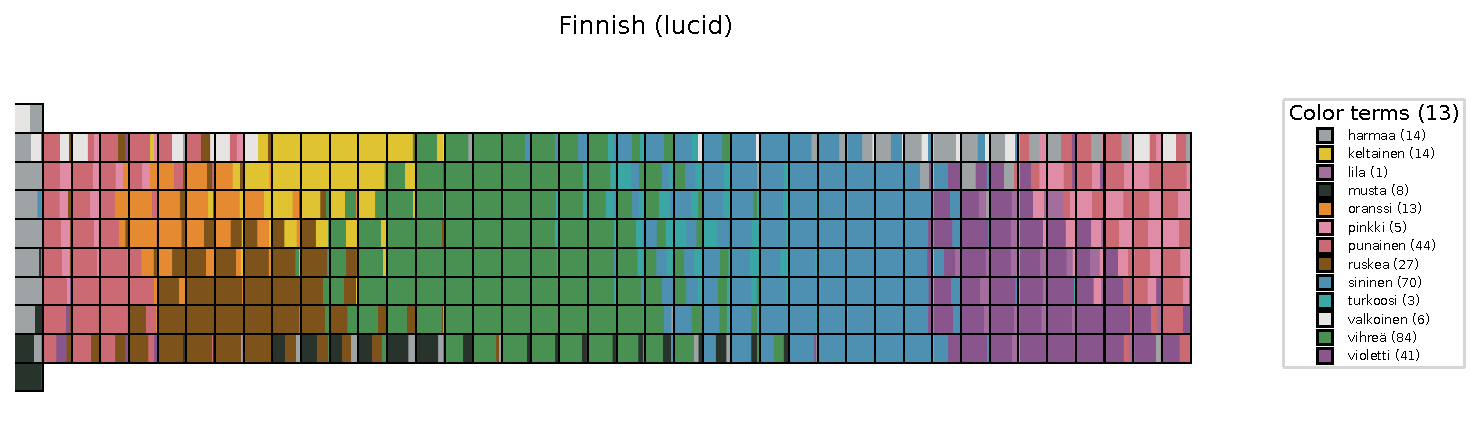
\includegraphics[page=1, width=\linewidth]{images/mode_maps/Finnish (lucid).pdf}
\caption[Proportion Maps (Arabic, Danish, Dutch, English, Finnish]{Proportion maps for Arabic, Danish, Dutch, English, Finnish and respective color terms.}
\label{fig:color_maps_1}
\end{figure}

\begin{figure}[htbp]
\centering
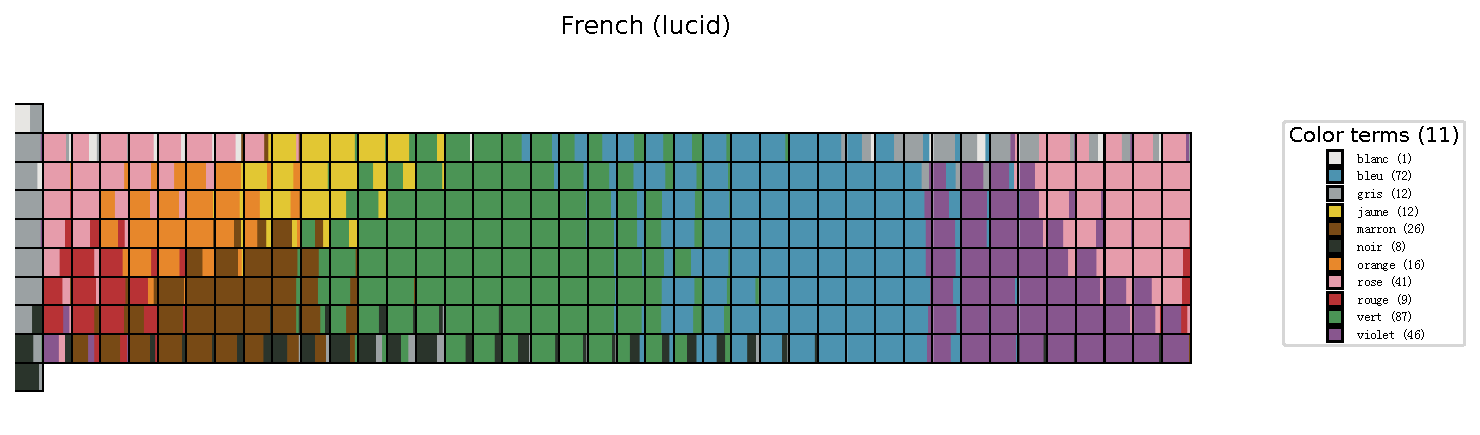
\includegraphics[page=1, width=\linewidth]{images/mode_maps/French (lucid).pdf}
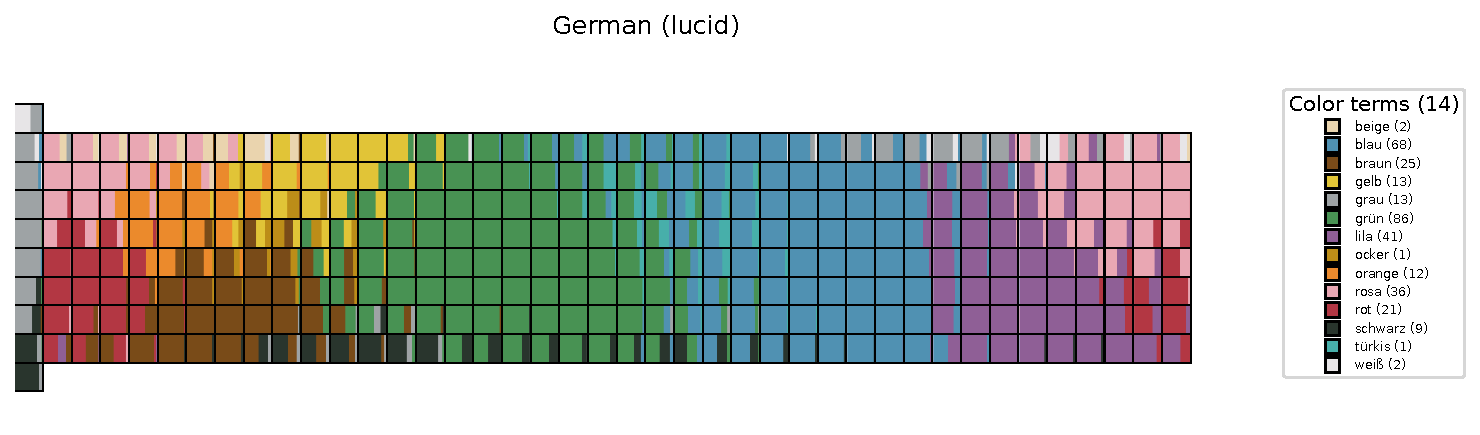
\includegraphics[page=1, width=\linewidth]{images/mode_maps/German (lucid).pdf}
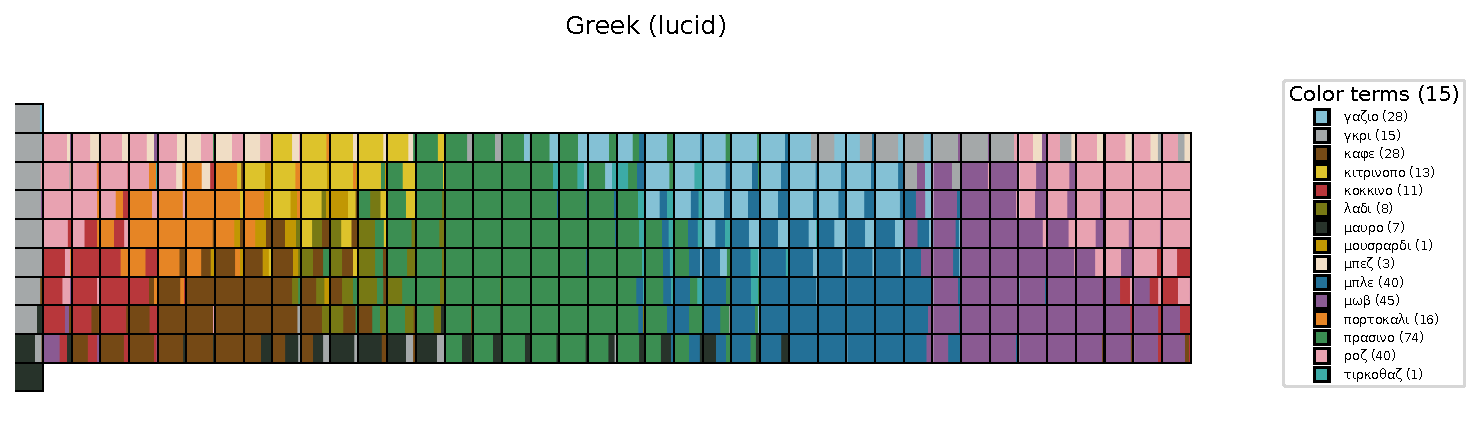
\includegraphics[page=1, width=\linewidth]{images/mode_maps/Greek (lucid).pdf}
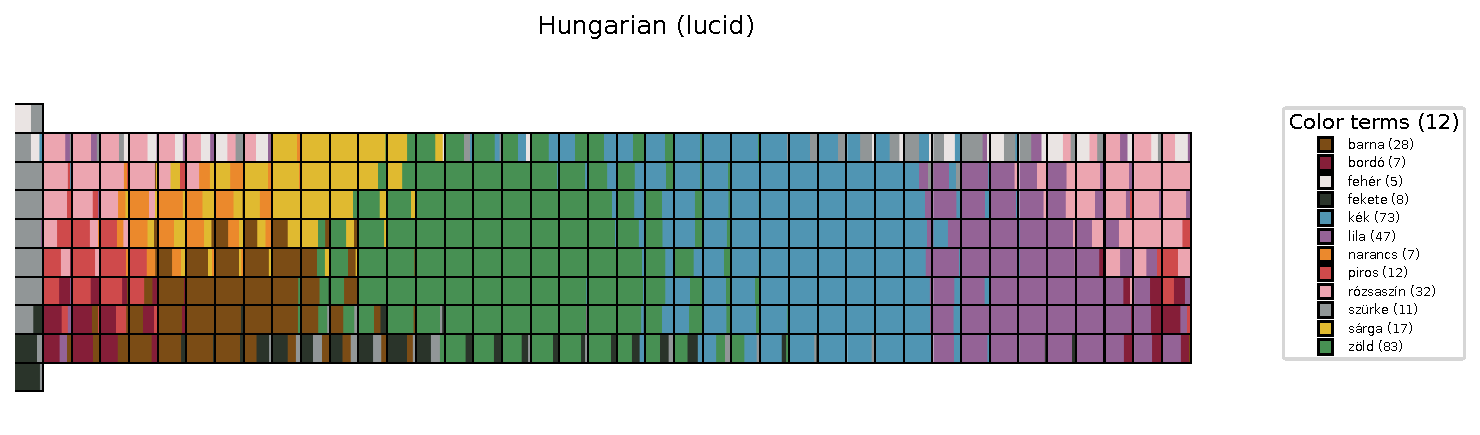
\includegraphics[page=1, width=\linewidth]{images/mode_maps/Hungarian (lucid).pdf}
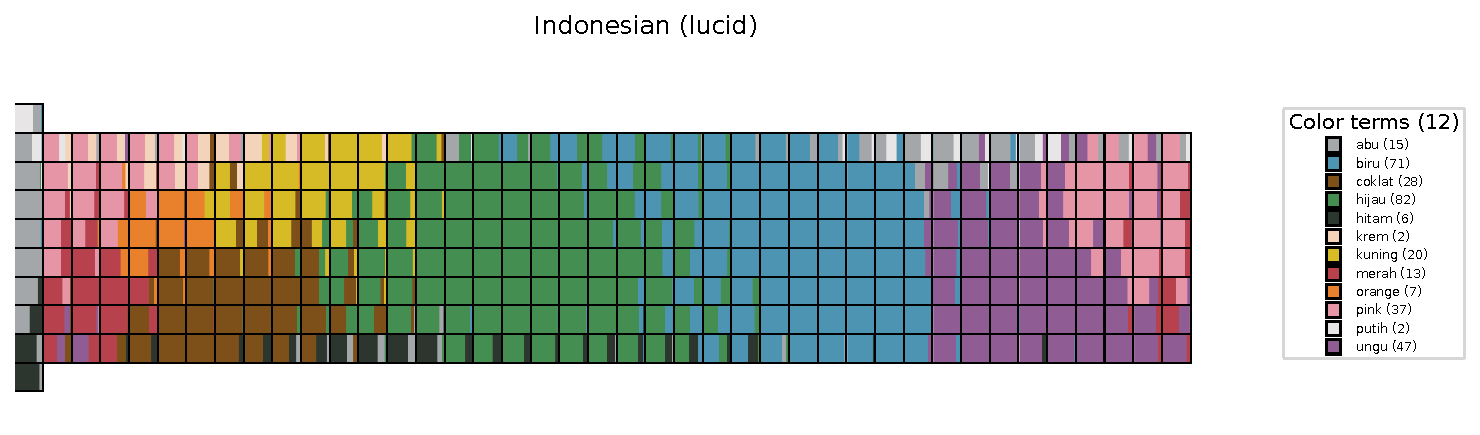
\includegraphics[page=1, width=\linewidth]{images/mode_maps/Indonesian (lucid).pdf}
\caption[Proportion Maps (French, German, Greek, Hungarian, Indonesian)]{Proportional maps for French, German, Greek, Hungarian, Indonesian and respective color terms.}
\label{fig:color_maps_2}
\end{figure}

\begin{figure}[htbp]
\centering
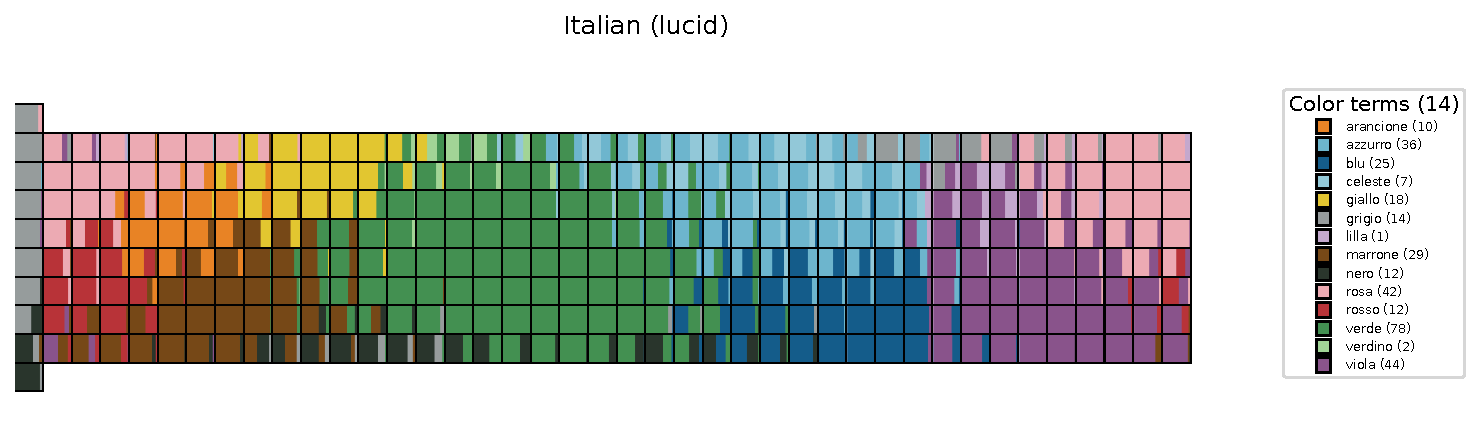
\includegraphics[page=1, width=\linewidth]{images/mode_maps/Italian (lucid).pdf}
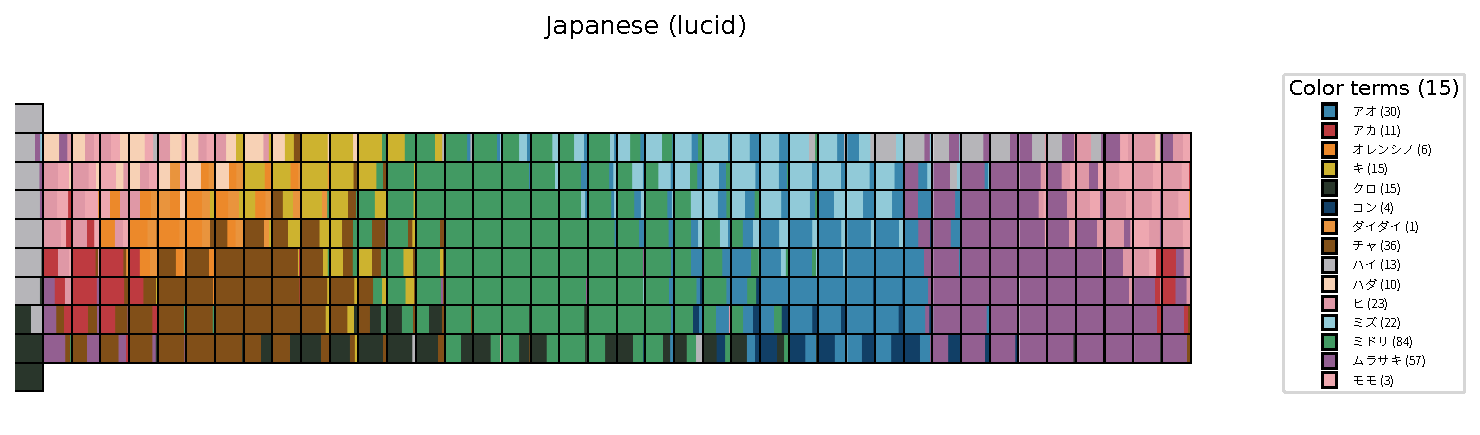
\includegraphics[page=1, width=\linewidth]{images/mode_maps/Japanese (lucid).pdf}
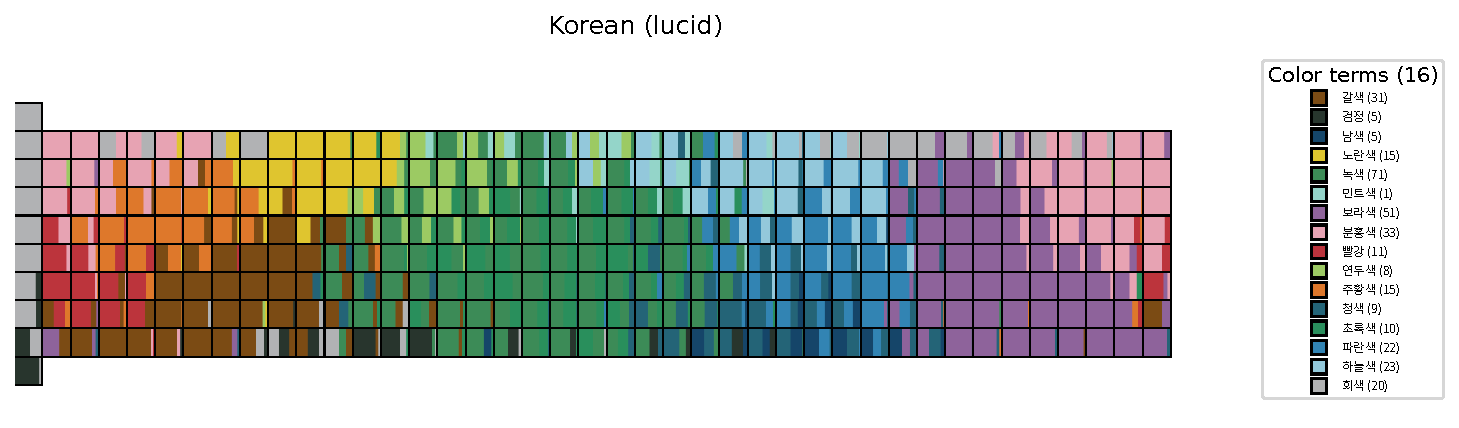
\includegraphics[page=1, width=\linewidth]{images/mode_maps/Korean (lucid).pdf}
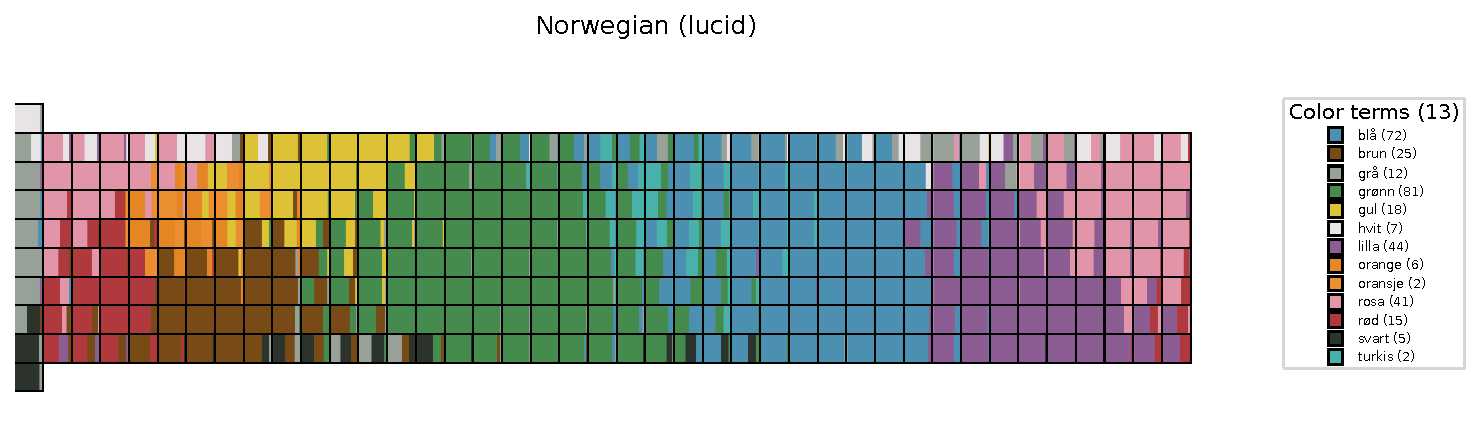
\includegraphics[page=1, width=\linewidth]{images/mode_maps/Norwegian (lucid).pdf}
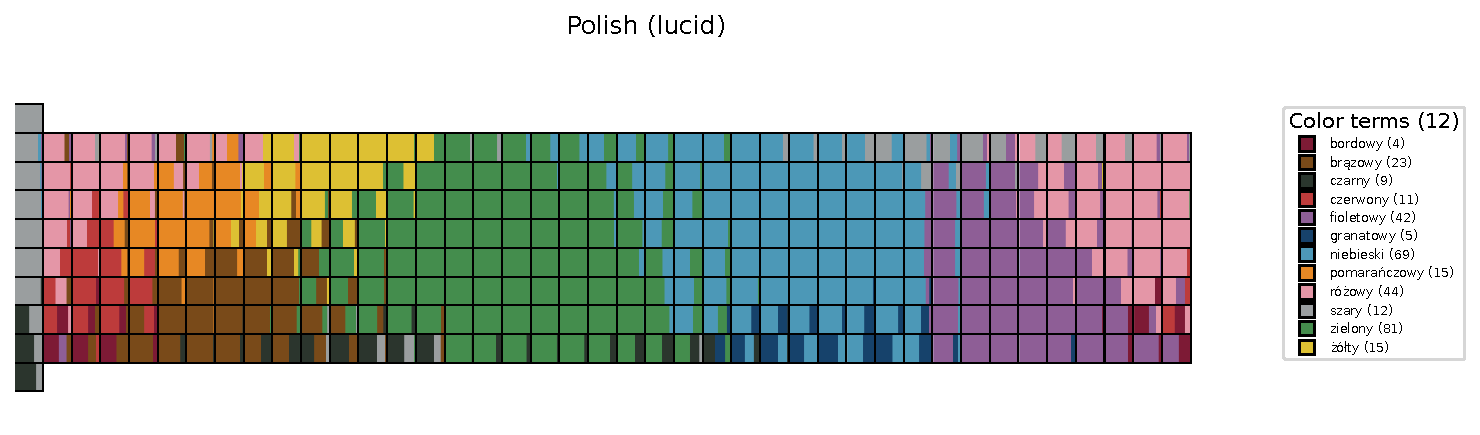
\includegraphics[page=1, width=\linewidth]{images/mode_maps/Polish (lucid).pdf}
\caption[Proportion Maps (Italian, Japanese, Korean, Norwegian, Polish)]{Proportional maps for Italian, Japanese, Korean, Norwegian, Polish and respective color terms.}
\label{fig:color_maps_3}
\end{figure}

\begin{figure}[htbp]
\centering
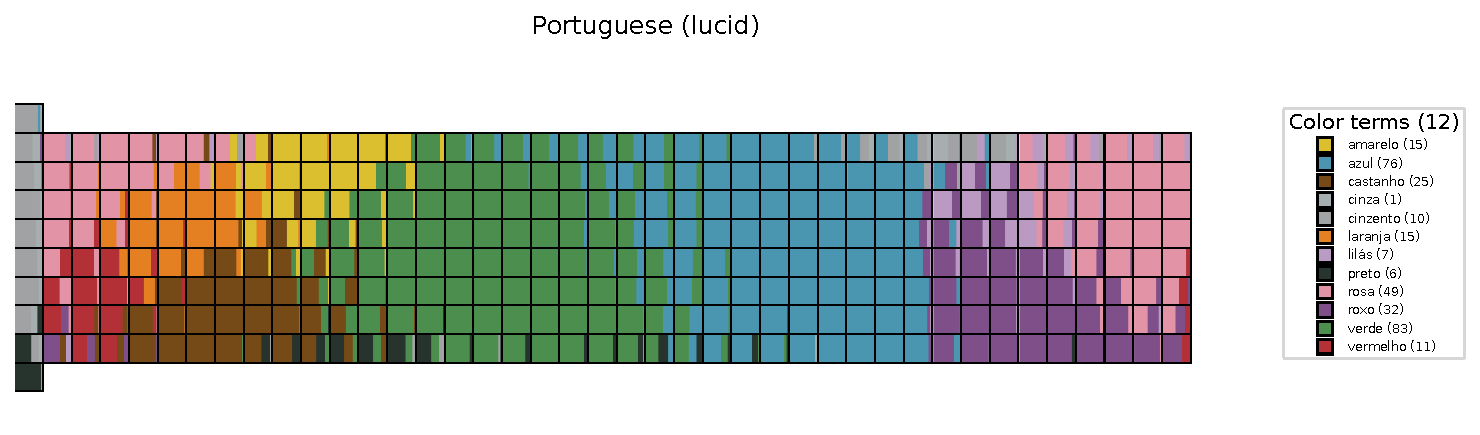
\includegraphics[page=1, width=\linewidth]{images/mode_maps/Portuguese (lucid).pdf}
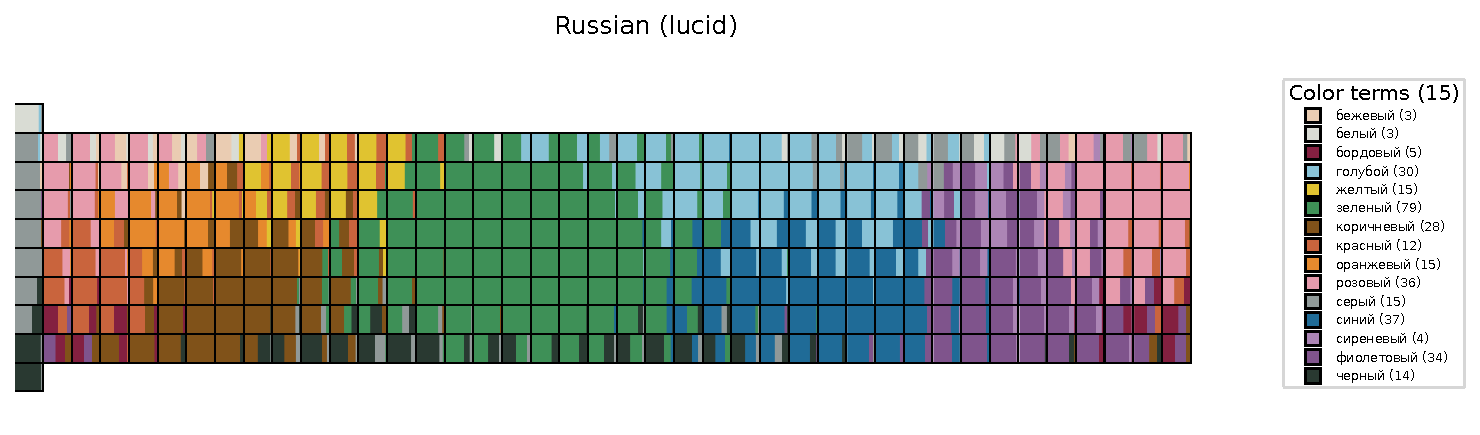
\includegraphics[page=1, width=\linewidth]{images/mode_maps/Russian (lucid).pdf}
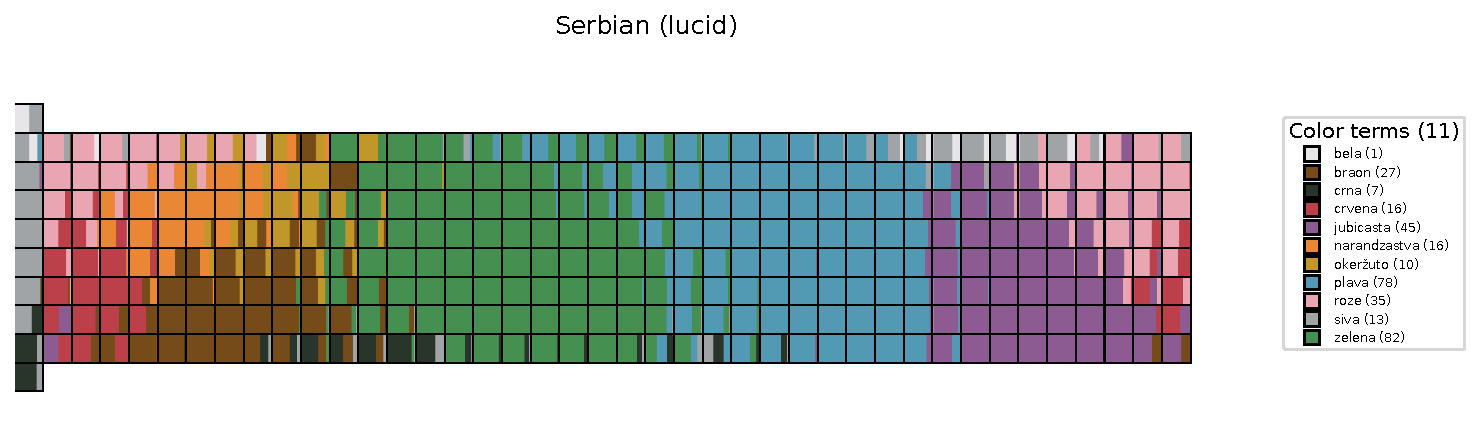
\includegraphics[page=1, width=\linewidth]{images/mode_maps/Serbian (lucid).pdf}
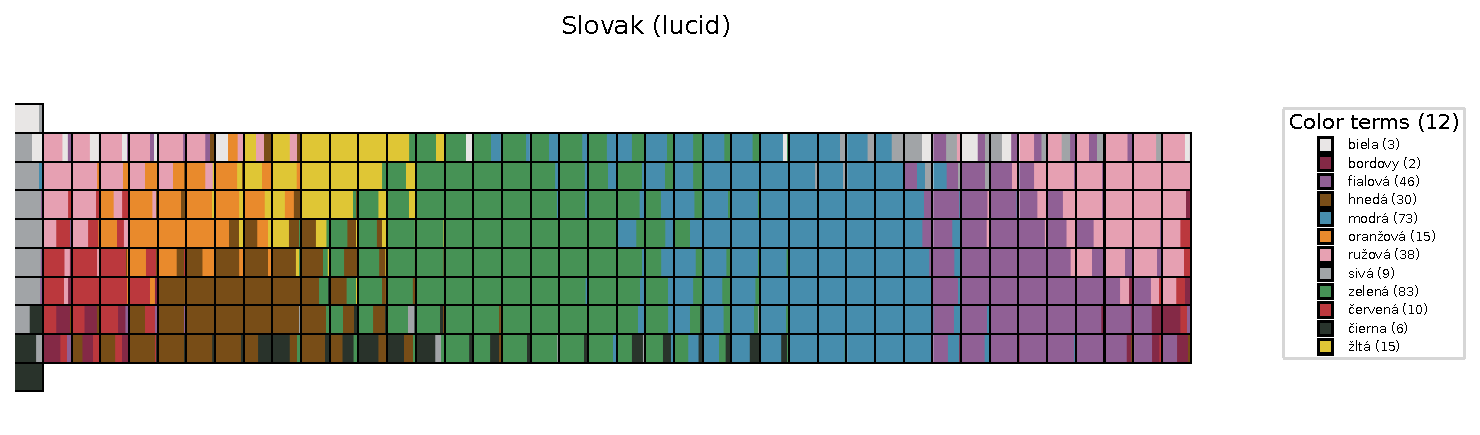
\includegraphics[page=1, width=\linewidth]{images/mode_maps/Slovak (lucid).pdf}
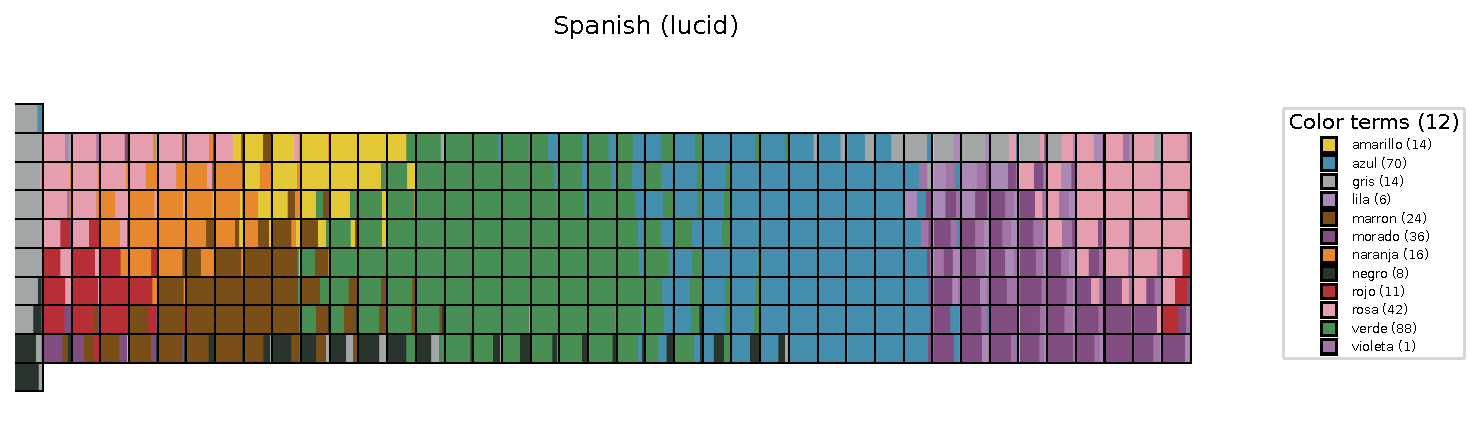
\includegraphics[page=1, width=\linewidth]{images/mode_maps/Spanish (lucid).pdf}
\caption[Proportion Maps (Russian, Serbian, Slovakian, Spanish)]{Proportional maps for Russian, Serbian, Slovakian, Spanish and respective color terms.}
\label{fig:color_maps_4}
\end{figure}

\begin{figure}[htbp]
\centering
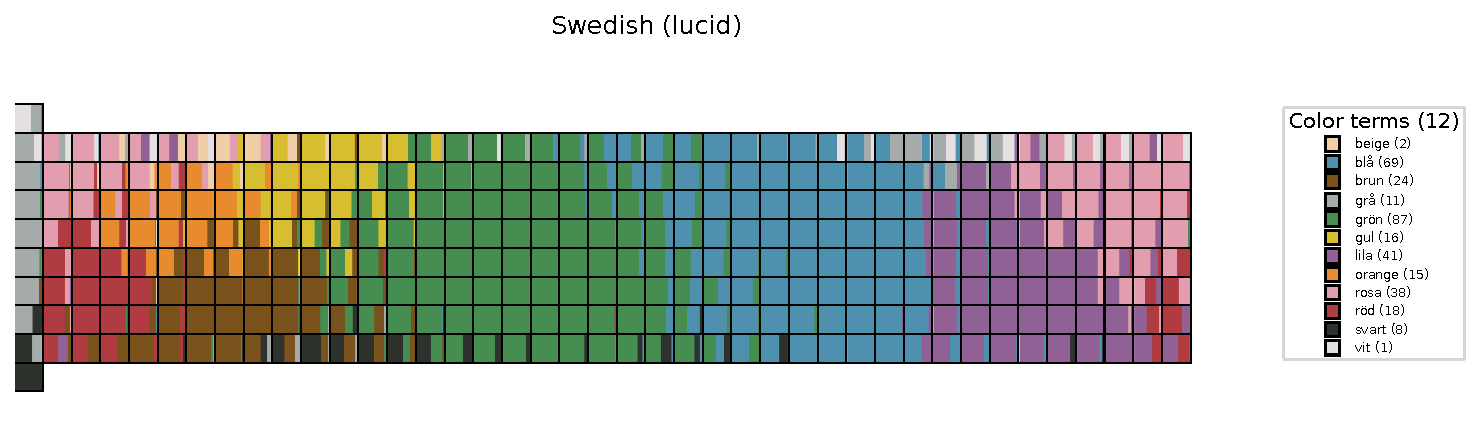
\includegraphics[page=1, width=\linewidth]{images/mode_maps/Swedish (lucid).pdf}
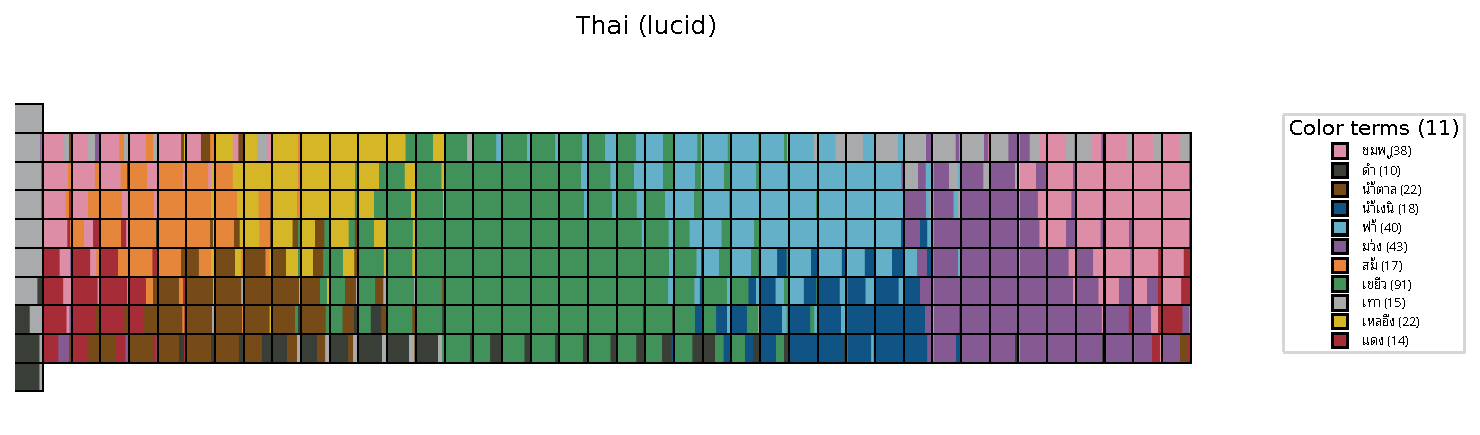
\includegraphics[page=1, width=\linewidth]{images/mode_maps/Thai (lucid).pdf}
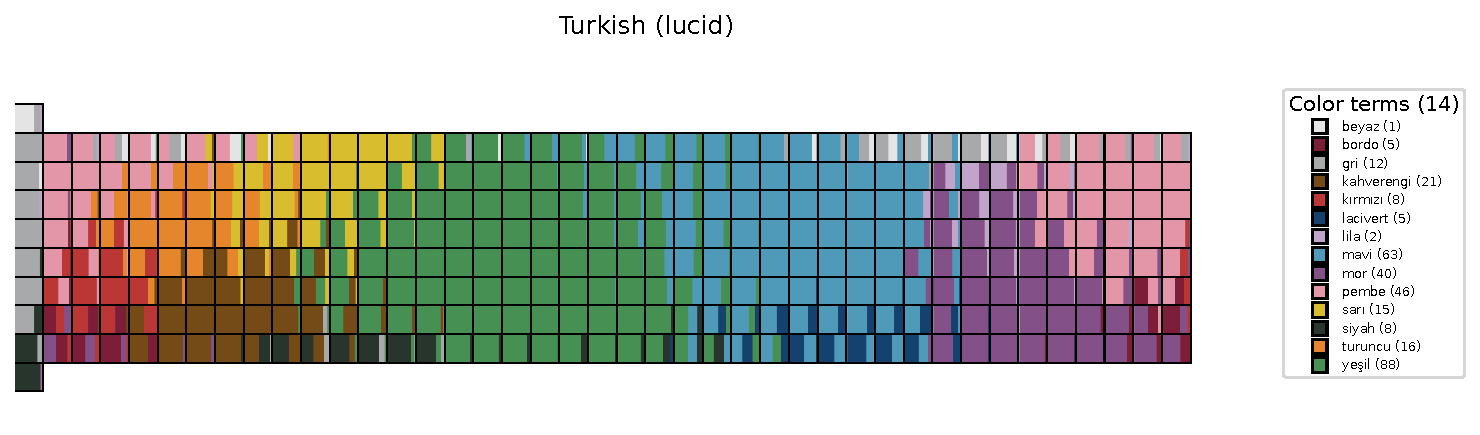
\includegraphics[page=1, width=\linewidth]{images/mode_maps/Turkish (lucid).pdf}
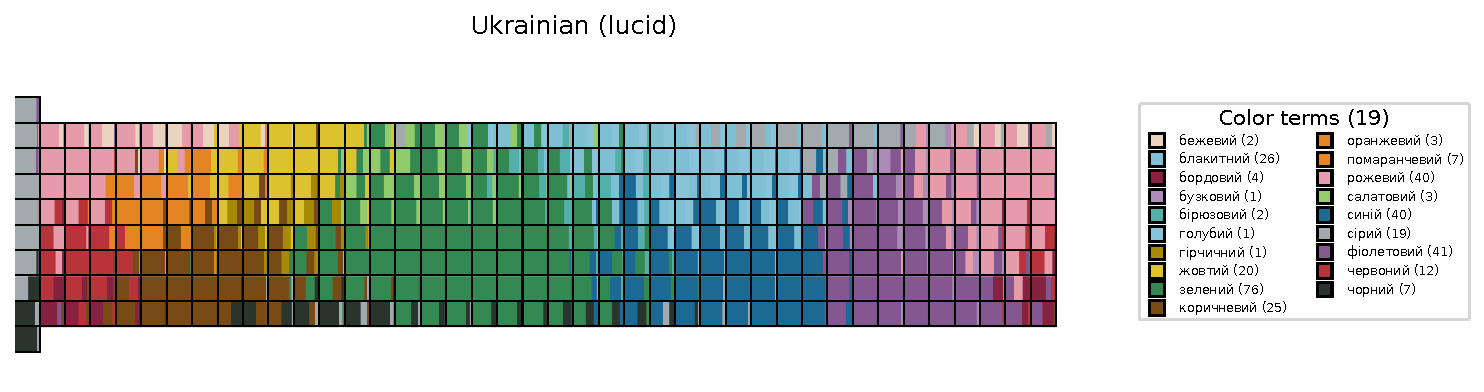
\includegraphics[page=1, width=\linewidth]{images/mode_maps/Ukrainian (lucid).pdf}
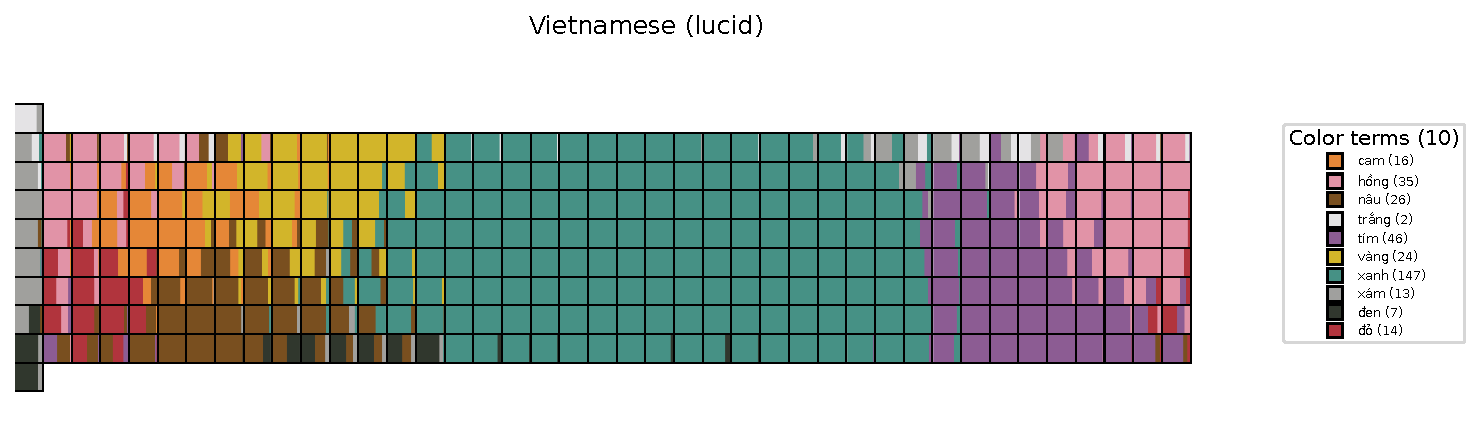
\includegraphics[page=1, width=\linewidth]{images/mode_maps/Vietnamese (lucid).pdf}
\caption[Proportion Maps (Swedish, Thai, Turkish, Ukrainian, Vietnamese)]{Proportional maps for Swedish, Thai, Turkish, Ukrainian, Vietnamese and respective color terms.}
\label{fig:color_maps_5}
\end{figure}


\subsection{Relations between languages}

\begin{figure}[h!t]
\centering
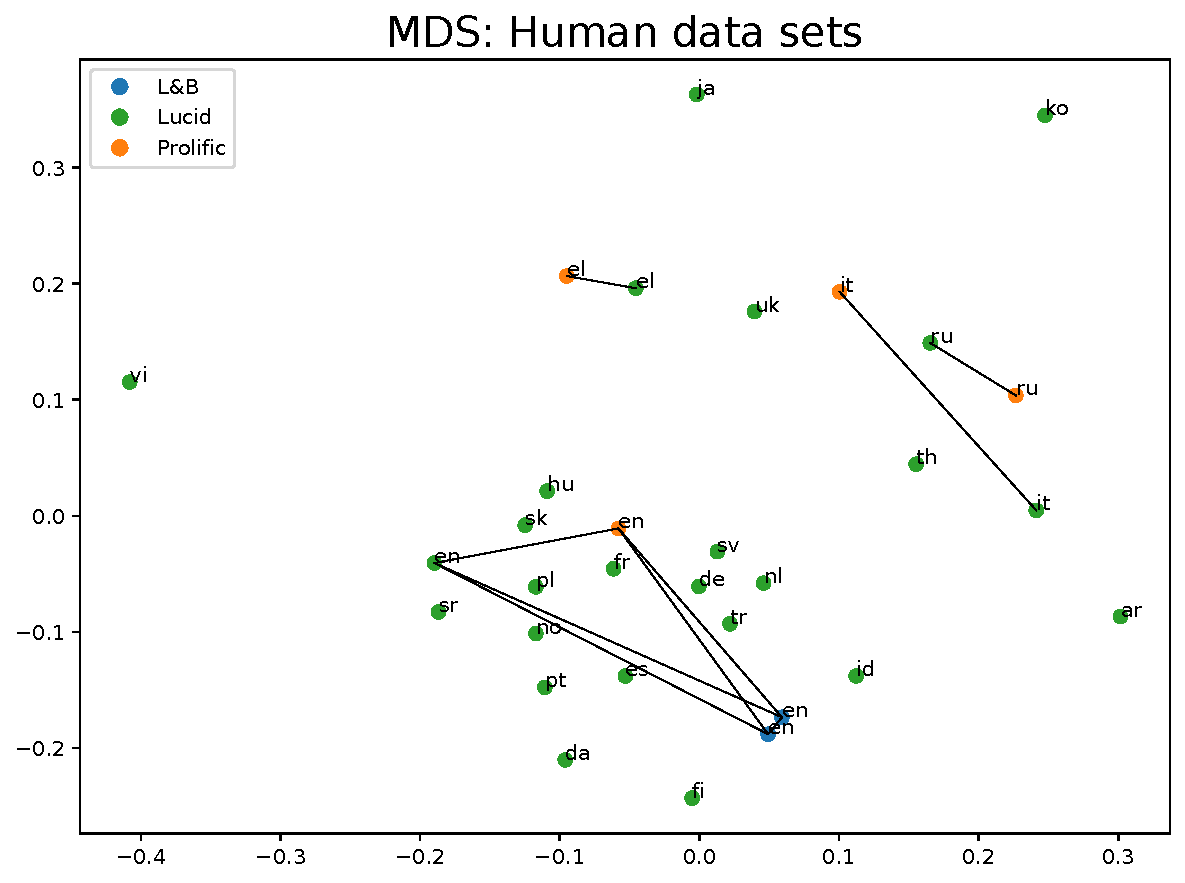
\includegraphics[page=1, width=0.49\linewidth]{images/MDS/mds_rand_index_human.pdf}
\hfill
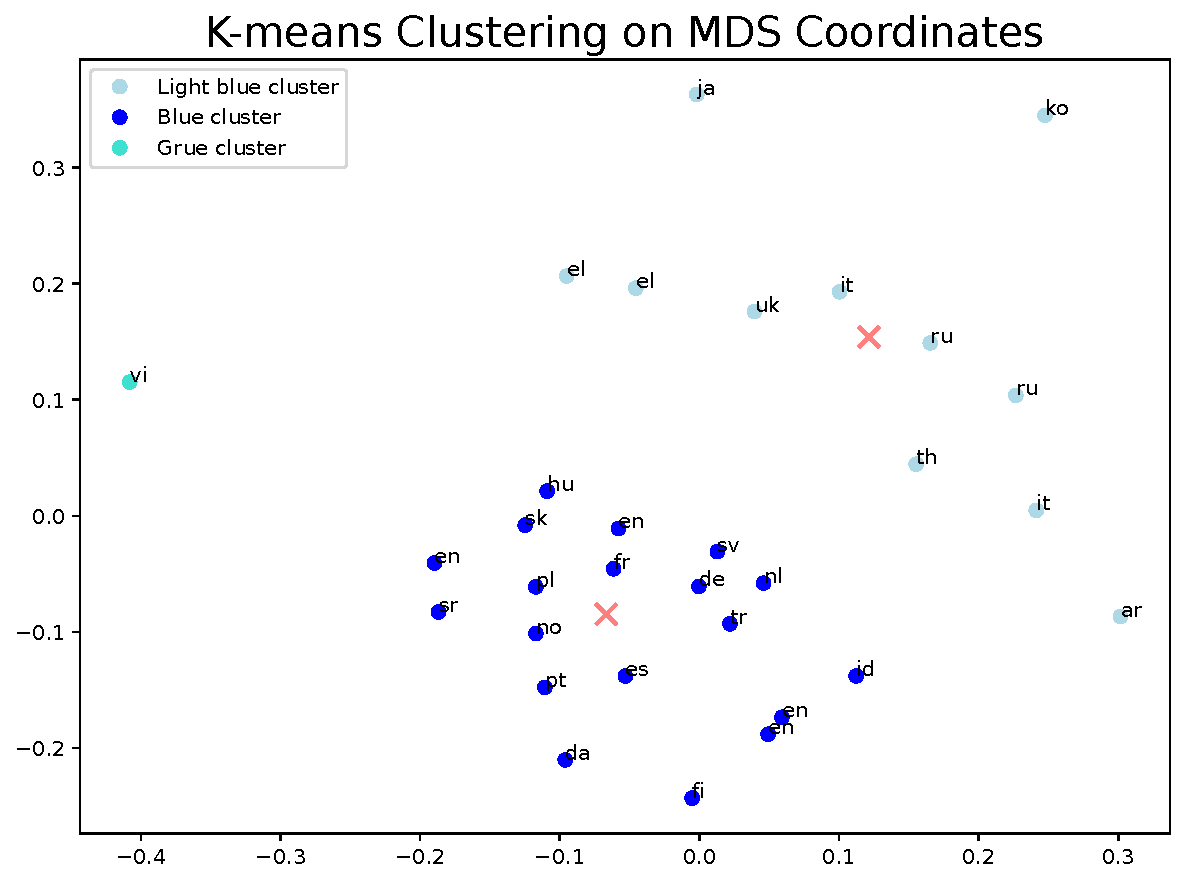
\includegraphics[page=1, width=0.49\linewidth]{images/MDS/kmeans_human.pdf}
\decoRule
\caption[MDS human data]{MDS human data. Left panel: MDS embedding based on the ARI matrix of human data (Lucid, Prolific, WCS) with lines connecting data points of the same language but different sources.
Right panel: K-means clustering (k=2) of MDS coordinates distinguishes two clusters: one representing languages with a distinct light blue category and another with a singular broad blue category.
The cluster centers are denoted by the red crosses.
Notably, Vietnamese, marked in a unique color, deviates due to its 'grue' category that merges green and blue hues.}
\label{fig:MDS_human}
\end{figure}



When observing the Rand Index Matrix directly, it is not possible to compare similarity and difference between color terms usage, as the Rand index simply provide overall distance score for each pair.
A multidimensional scaling (MDS) approach may be used to reveal the latent structure of the Rand matrix \parencite{shepard1980multidimensional}. Embedding the rand index values as a dissimilarity matrix into an MDS visually reveals the clustering of different languages and give more intuitive understanding about the similarities and dissimilarities across languages (Fig. \ref{fig:MDS_human}).
As expected, data of the same languages but different recruiters (el, ru, it, en) are mapped relatively close to each other. 
Furthermore, the constellation of languages in the MDS appears to be divided into three clusters.
First, Vietnamese is a special outlier placed in the periphery. This might be due to the large xanh category combining blue and green (grue) and a low overall number of 5.96 color terms in the lexicon (calculated as the exponent of the global entropy).
Second, a group of languages namely Hungarian, Slovakian, Serbian, Norwegian, Polish, French, Portuguese, Danish, Spanish, Swedish, Dutch, German, Turkish, Indonesian and Finish form a cluster which generally aligns strongly with the English lexicon. 
All these lexicon do distinguish between green and blue and have a mean of 8.06 [7.40, 8.73] color terms.
Additional categories to the eleven BCT are not major categories.
I will refer to this cluser as the blue cluster.
However, within the cluster different grouping tendencies can be described. 
Danish and Finish located at one extreme of the cluster both share a large red category (Finnish: punainen, Danish: rød) instead of differentiated between red and pink which is very small for Danish and Finnish. For both languages we detected a high usage of compound words (e.g. Finish: light red = vaaleanpunainen, Danish:light red = lys rød). The large red category result due to our heuristics to resolve compound words by replacing them with the base. 
Hungarian is located on the opposite side of the cluster. Reason for this might be an additional small category for dark red - bordó.


The third cluster consists of Greek, Ukraine, Japanese, Italian, Russian, Thai and Arabic.
A distinctive characteristic of these languages is the universal categorization of a 'light blue' hue, accompanied by an average lexicon comprising 10.70 [8.59, 12.81] color terms, indicative for a broadened chromatic vocabulary.
In the following I will refer to this groupe as the “light blue” cluster.
Languages of this cluster contain additional color categories in different parts of color space which makes it hard to categorize the relative position within the language.

K-means algorithm of the \textit{sklearn} library successfully distinguishes two clusters but fails to detect Vietnamese as a third cluster presumably because it is just one language (Fig. \ref{fig:MDS_human}).
The light blue cluster has a mean bootstrapped ARI to the English data of .59 (sd=.07) whereas the blue category has a higher ARI of .75 (sd=.06).



